\chapter{Background Estimation and Systematics}

\section{Introduction}

\section{QCD Background}

\subsection{Electroweak Background}

Electroweak processes can have real MET due to neutrinos which are not
detected by CMS. There are two components to the electroweak background:
$W\rightarrow e\nu$, where the electron is misidentified as a photon and 
$\gamma Z\rightarrow\gamma\nu\nu$, which has a real photon and real MET. \\

The $W\rightarrow e\nu$ background is estimated by measuring the electron/photon
misidentification rate in data. \\

The $\gamma Z\rightarrow\gamma\nu\nu$ background is estimated from Monte Carlo.

\section{Electron/Photon Fake Rate}

Measuring the fraction of electrons that are misidentified as photons is
important for estimating the background coming from $W\rightarrow e\nu$ events
where the electron is misidentified as a photon. \\

With a fake rate, $f_{e\rightarrow\gamma}$, and given a true number of
$Z\rightarrow ee$ events, $N_{Z}$, the number of events in the ee sample is
given by $N_{ee} = (1 - f_{e\rightarrow\gamma})^{2}N_{Z}$. And the number of
events in the e$\gamma$ is given by $N_{e\gamma} = 2[f_{e\rightarrow\gamma}(1 -
f_{e\rightarrow\gamma})]N_{Z}$. With measurements of $N_{ee}$ and $N_{e\gamma}$
the fake rate can be determined as $f_{e\rightarrow\gamma} =
N_{e\gamma}/(2N_{ee} + N_{e\gamma})$. \\

The fake rate is measured using an ee sample and an e$\gamma$ sample from data.
Electrons are selected using the same requirements as photons, but with a pixel
seed required (rather than no pixel seed). The number of $Z\rightarrow ee$
events in each sample is determined by fitting a Crystal Ball function with a
linear background assumption (Figure \ref{fig:Zee_Fit}). There is no significant
difference in the yields if a constsnt or quadratic background shape is used. \\

\begin{figure}
\begin{center}
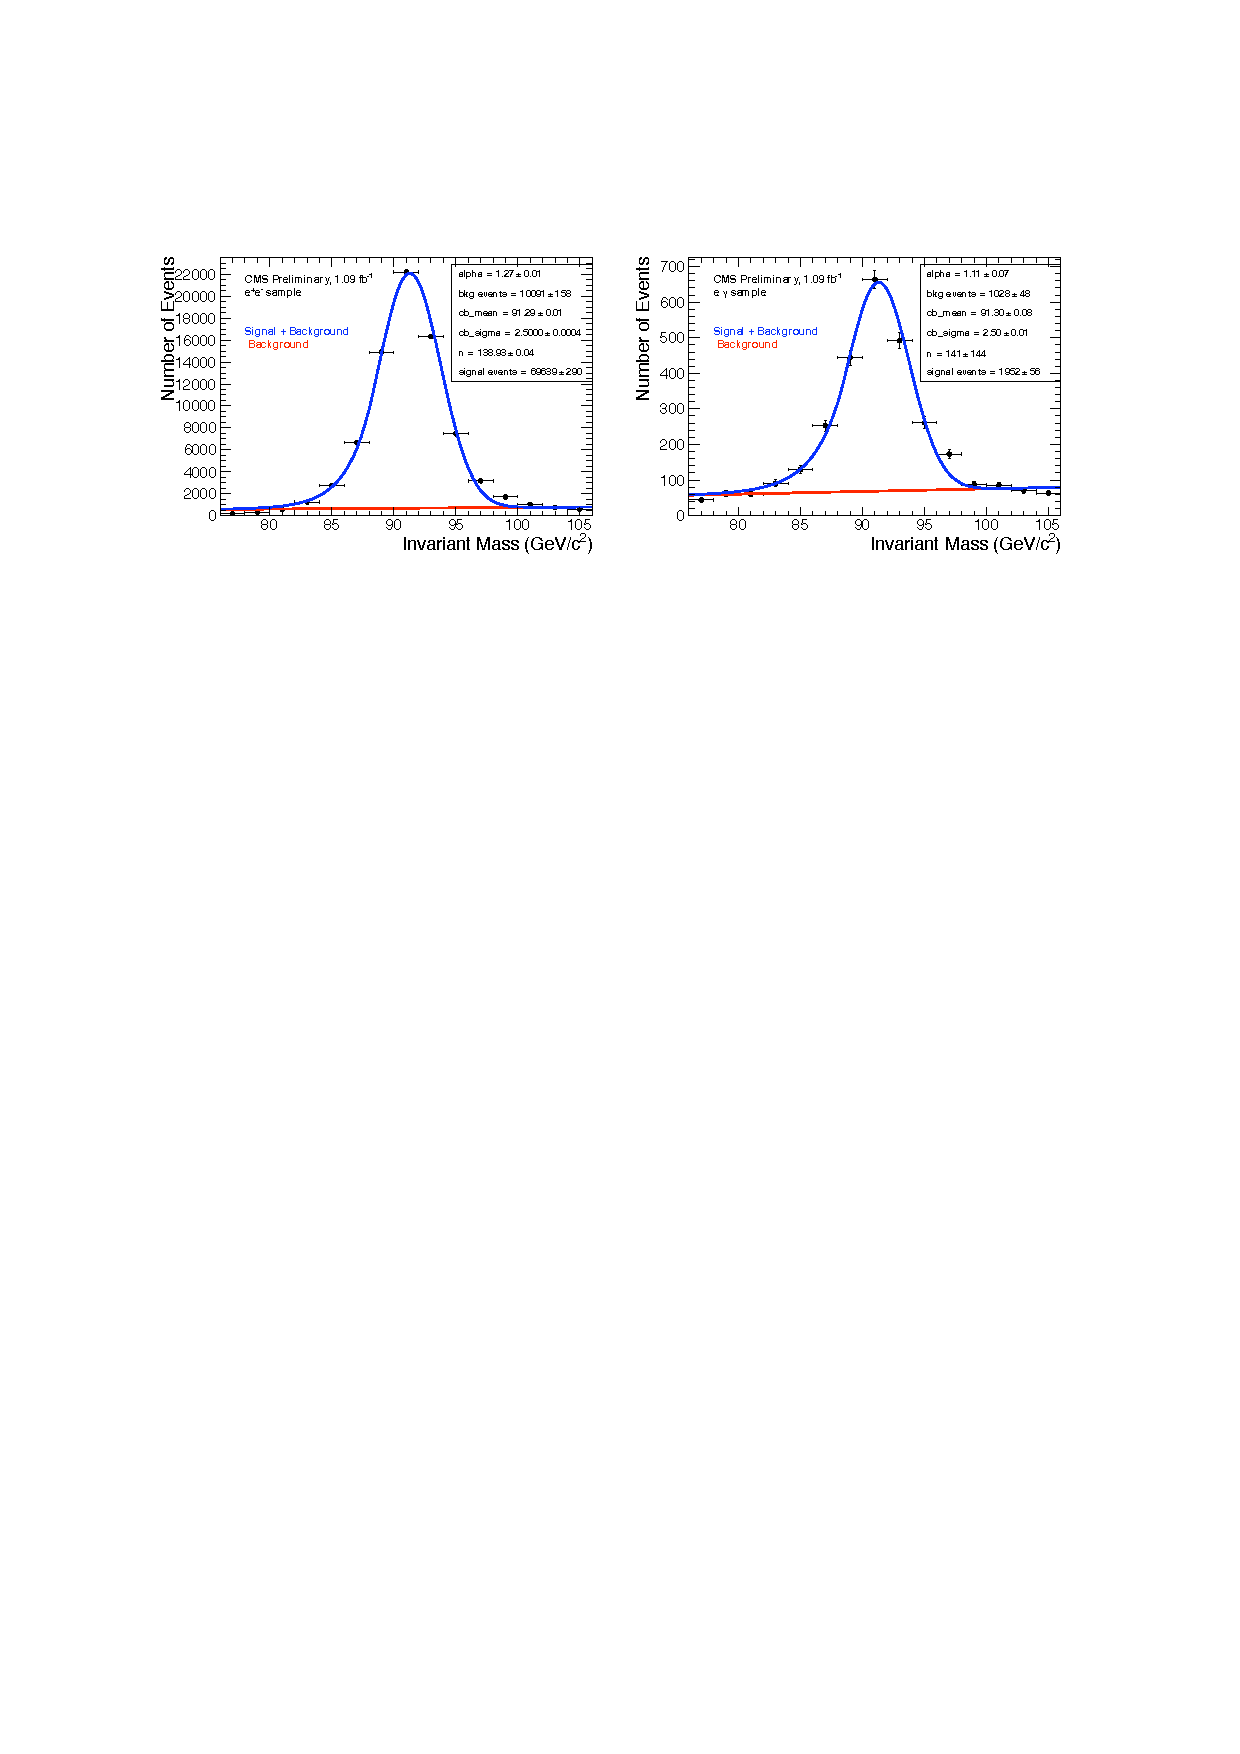
\includegraphics{Zee_Fit.pdf}
\end{center}
\caption{The invariant mass of ee and e$\gamma$ candidates. The Z peak is fitted
using a Crystal Ball function and a linear background.}
\label{fig:Zee_Fit}
\end{figure}

The fit of the Z peak in the ee sample yields $69639 \pm 290$ Z events. Fitting
the Z peak in the e$\gamma$ sample yield $1952\pm56$ Z events. From these
numbers the misidentification rate is $f_{e\rightarrow\gamma} = 0.014\pm0.004$.
This number varies little as a function of e or $\gamma$ $\pT$. Based on the
variations with $\pT$ a systematic uncertainty of 0.002 is assigned to
$f_{e\rightarrow\gamma}$. 

\section{GGM SUSY Scan}

\section{Systematic Uncertainties}
